\chapter{Results}

\begin{figure}[H]
    \centering
    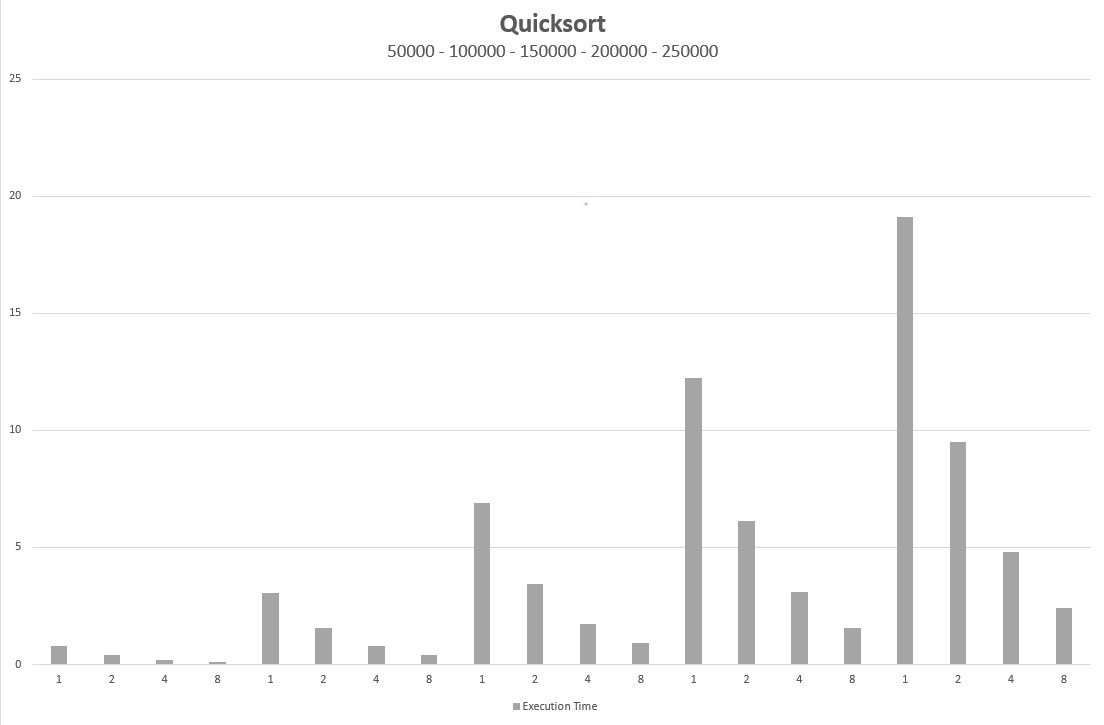
\includegraphics[width=0.8\textwidth]{graphics/Quicksort.jpg}
    \label{fig:Quicksort}
\end{figure}
\begin{table}[H]
    \centering
    \begin{tabular}{|l|l|l|l|l|}\hline
        Elements & Threads & Execution Time & Speedup & Efficiency \\\hline
        50000 & 1 & 0.775689 & 1 & 1 \\
        50000 & 2 & 0.400874 & 1.934994537 & 0.967497268\\
        50000 & 4 & 0.210868 & 3.678552459 & 0.919638115\\
        50000 & 8 & 0.128504 & 6.036302372 & 0.754537796\\\hline
        100000 & 1 & 3.056718 & 1 & 1\\
        100000 & 2 & 1.553926 & 1.967093671 & 0.983546836\\
        100000 & 4 & 0.78471 & 3.895347326 & 0.973836831\\
        100000 & 8 & 0.415125 & 7.36336766 & 0.920420958\\\hline
        150000 & 1 & 6.898998 & 1 & 1\\
        150000 & 2 & 3.447924 & 2.000913593 & 1.000456797\\
        150000 & 4 & 1.739329 & 3.966470978 & 0.991617745\\
        150000 & 8 & 0.901691 & 7.651177621 & 0.956397203\\\hline
        200000 & 1 & 12.246717 & 1 & 1\\
        200000 & 2 & 6.124838 & 1.999516885 & 0.999758443\\
        200000 & 4 & 3.0787 & 3.977885796 & 0.994471449\\
        200000 & 8 & 1.566689 & 7.816941971 & 0.977117746\\\hline
        250000 & 1 & 19.125711 & 1 & 1\\
        250000 & 2 & 9.491847 & 2.014961998 & 1.007480999\\
        250000 & 4 & 4.794321 & 3.989242898 & 0.997310725\\
        250000 & 8 & 2.421326 & 7.898858312 & 0.987357289\\\hline
        
        
    \end{tabular}
    \label{tab:Quicksort_Table}
\end{table}

\begin{figure}[H]
    \centering
    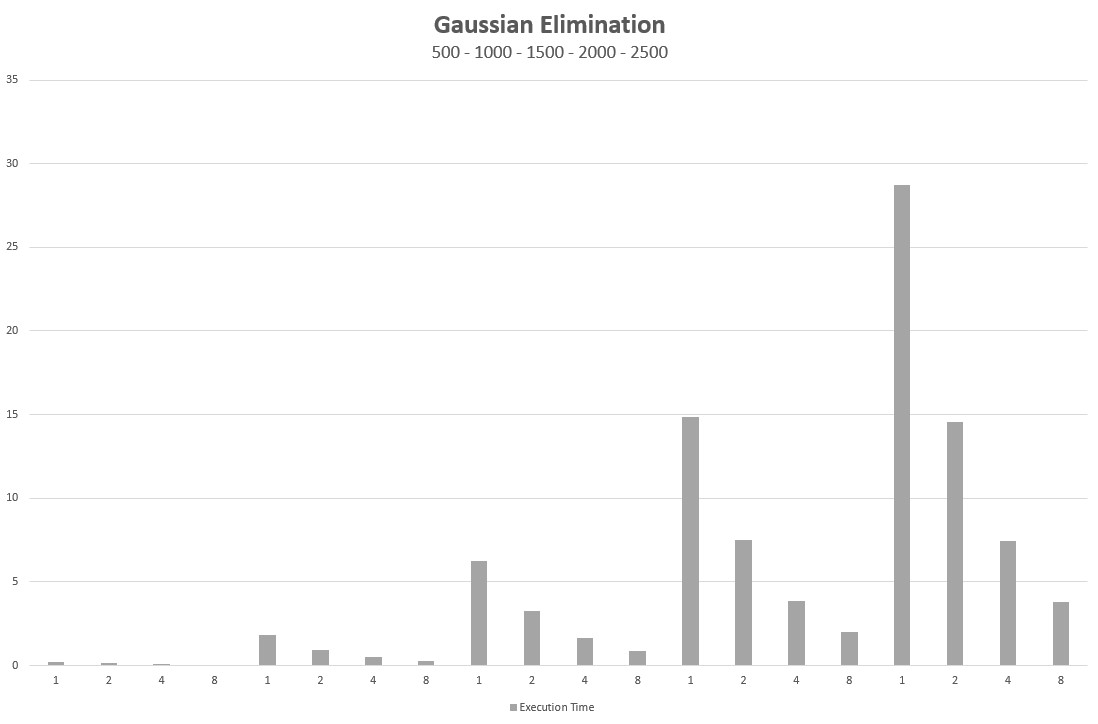
\includegraphics[width=0.8\textwidth]{graphics/Gaussian.jpg}
    \label{fig:Gaussian}
\end{figure}
\begin{table}[H]
    \centering
    \begin{tabular}{|l|l|l|l|l|}\hline
        Elements & Threads & Execution Time & Speedup & Efficiency \\\hline
        500 & 1 & 0.234272 & 1 & 1 \\
        500 & 2 & 0.12492 & 1.875376241 & 0.93768812\\
        500 & 4 & 0.066969 & 3.498215592 & 0.874553898\\
        500 & 8 & 0.038337 & 6.110858961 & 0.76385737\\\hline
        1000 & 1 & 1.831963 & 1 & 1\\
        1000 & 2 & 0.937822 & 1.953422931 & 0.976711466\\
        1000 & 4 & 0.486209 & 3.767850862 & 0.941962716\\
        1000 & 8 & 0.261493 & 7.005782182 & 0.875722773\\\hline
        1500 & 1 & 6.269111 & 1 & 1\\
        1500 & 2 & 3.258832 & 1.923729422 & 0.961864711\\
        1500 & 4 & 1.650532 & 3.798236569 & 0.949559142\\
        1500 & 8 & 0.859762 & 7.291681884 & 0.911460236\\\hline
        2000 & 1 & 14.873661 & 1 & 1\\
        2000 & 2 & 7.525389 & 1.976464074 & 0.988232037\\
        2000 & 4 & 3.859083 & 3.854195673 & 0.963548918\\
        2000 & 8 & 1.978362 & 7.518169577 & 0.939771197\\\hline
        2500 & 1 & 28.706882 & 1 & 1\\
        2500 & 2 & 14.568114 & 1.970528375 & 0.985264187\\
        2500 & 4 & 7.419112 & 3.869315088 & 0.967328772\\
        2500 & 8 & 3.796063 & 7.562277549 & 0.945284694\\\hline
    \end{tabular}
    \label{tab:Gaussian_Table}
\end{table}

\begin{figure}[H]
    \centering
    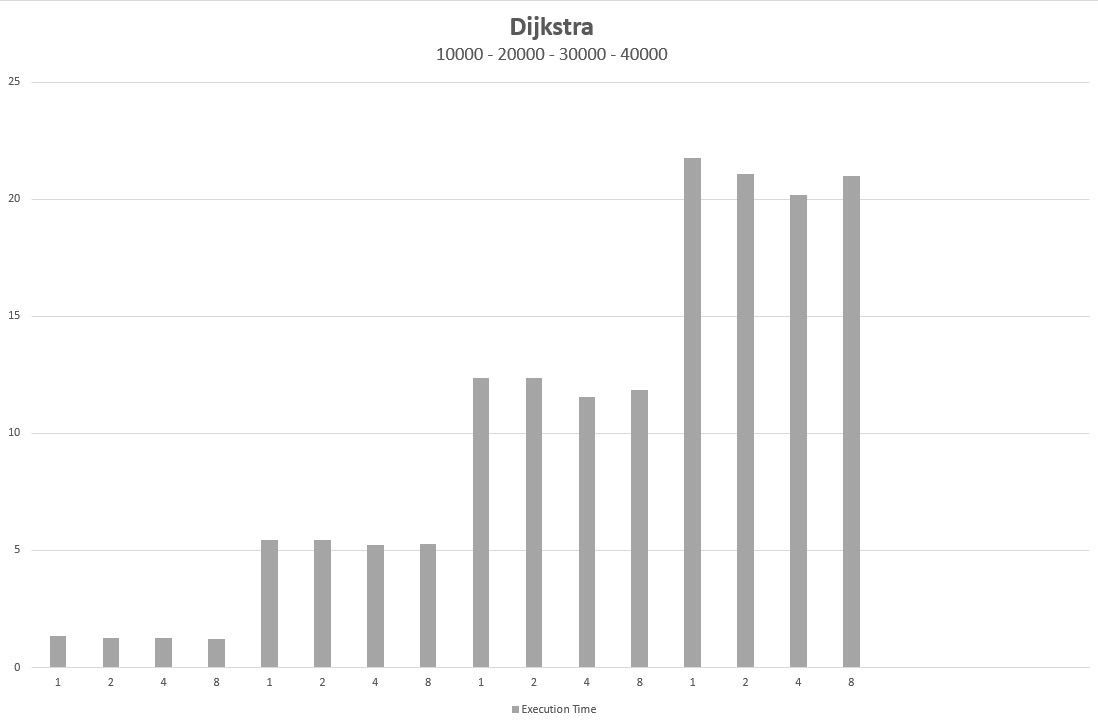
\includegraphics[width=0.8\textwidth]{graphics/Dijkstra.jpg}
    \label{fig:Dijkstra}
\end{figure}
\begin{table}[H]
    \centering
    \begin{tabular}{|l|l|l|l|l|}\hline
        Elements & Threads & Execution Time & Speedup & Efficiency \\\hline
        10000 & 1 & 1.338108 & 1 & 1 \\
        10000 & 2 & 1.256426 & 1.065011389 & 0.532505695\\
        10000 & 4 & 1.243389 & 1.076178091 & 0.269044523\\
        10000 & 8 & 1.206436 & 1.109141305 & 0.138642663\\\hline
        20000 & 1 & 5.431619 & 1 & 1\\
        20000 & 2 & 5.462286 & 0.994385684 & 0.497192842\\
        20000 & 4 & 5.236015 & 1.037357418 & 0.259339354\\
        20000 & 8 & 5.273222 & 1.030037992 & 0.128754749\\\hline
        30000 & 1 & 12.358053 & 1 & 1\\
        30000 & 2 & 12.38346 & 0.997948312 & 0.498974156\\
        30000 & 4 & 11.536593 & 1.071204731 & 0.267801183\\
        30000 & 8 & 11.849864 & 1.04288564 & 0.130360705\\\hline
        40000 & 1 & 21.745368 & 1 & 1\\
        40000 & 2 & 21.083123 & 1.031411143 & 0.515705572\\
        40000 & 4 & 20.171716 & 1.078012798 & 0.269503199\\
        40000 & 8 & 20.985627 & 1.036202921 & 0.129525365\\\hline
        

    \end{tabular}
    \label{tab:Dijkstra_Table}
\end{table}

\begin{figure}[H]
    \centering
    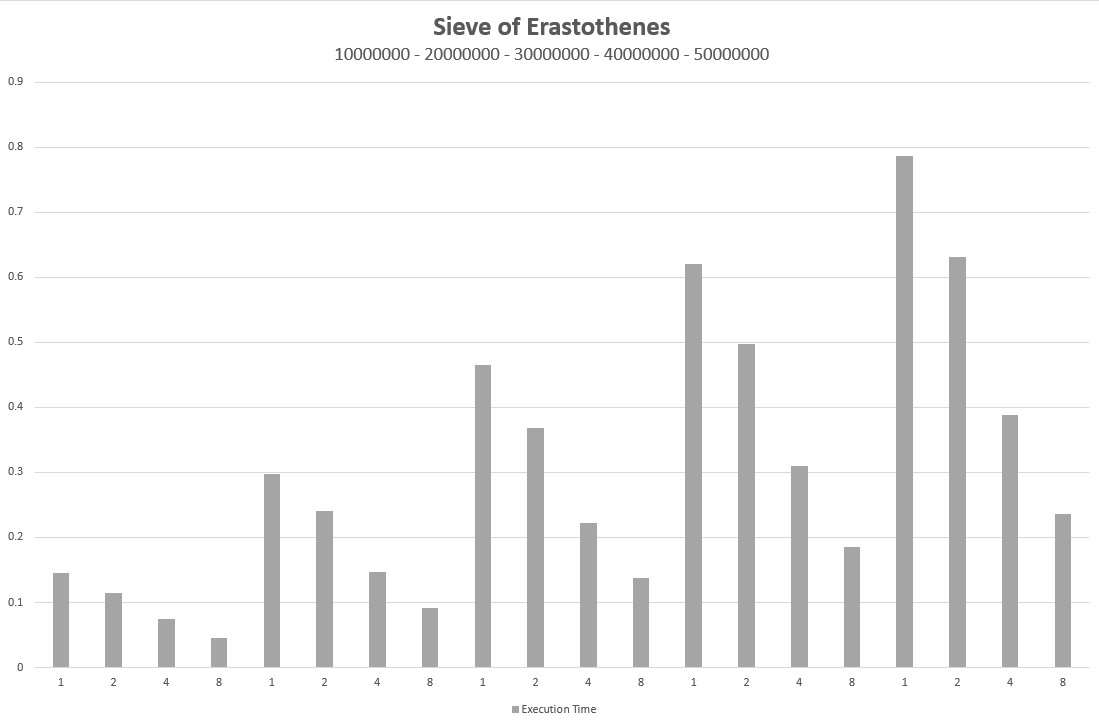
\includegraphics[width=0.8\textwidth]{graphics/Sieve.jpg}
    \label{fig:Sieve}
\end{figure}
\begin{table}[H]
    \centering
    \begin{tabular}{|l|l|l|l|l|}\hline
        Elements & Threads & Execution Time & Speedup & Efficiency \\\hline
        10000000 & 1 & 0.145243 & 1 & 1 \\
        10000000 & 2 & 0.114836 & 1.264786304 & 0.632393152\\
        10000000 & 4 & 0.074409 & 1.951954737 & 0.487988684\\
        10000000 & 8 & 0.045131 & 3.218253529 & 0.402281691\\\hline
        20000000 & 1 & 0.297384 & 1 & 1\\
        20000000 & 2 & 0.240418 & 1.236945653 & 0.618472826\\
        20000000 & 4 & 0.146255 & 2.033325356 & 0.508331339\\
        20000000 & 8 & 0.091809 & 3.23915956 & 0.404894945\\\hline
        30000000 & 1 & 0.464699 & 1 & 1\\
        30000000 & 2 & 0.368692 & 1.260398924 & 0.630199462\\
        30000000 & 4 & 0.221657 & 2.096477892 & 0.524119473\\
        30000000 & 8 & 0.138072 & 3.365628078 & 0.42070351\\\hline
        40000000 & 1 & 0.620618 & 1 & 1\\
        40000000 & 2 & 0.496802 & 1.24922605 & 0.624613025\\
        40000000 & 4 & 0.309458 & 2.005499939 & 0.501374985\\
        40000000 & 8 & 0.184713 & 3.359904284 & 0.419988035\\\hline
        50000000 & 1 & 0.786157 & 1 & 1\\
        50000000 & 2 & 0.631426 & 1.245050093 & 0.622525046\\
        50000000 & 4 & 0.388373 & 2.02423186 & 0.506057965\\
        50000000 & 8 & 0.236264 & 3.327451495 & 0.415931437\\\hline
    \end{tabular}
    \label{tab:Sieve_Table}
\end{table}




